\documentclass[8pt]{extarticle}
\title{}
\author{Avinash Iyer}
\date{}
\usepackage[shortlabels]{enumitem}

%font setup
%
%\usepackage[math]{anttor}

%paper setup
\usepackage{geometry}
\geometry{letterpaper, portrait, margin=1in}
\usepackage{fancyhdr}

%symbols
\usepackage{amsmath}
\usepackage{mathtools}
\usepackage{amssymb}
\usepackage{hyperref}
\usepackage{gensymb}

\usepackage[T1]{fontenc}
\usepackage[utf8]{inputenc}

%chemistry stuff
\usepackage[version=4]{mhchem}
\usepackage{chemfig}

%plotting
\usepackage{pgfplots}
\usepackage{tikz}
\usetikzlibrary{positioning}

%\usepackage{natbib}

%graphics stuff
\usepackage{graphicx}
\graphicspath{ {./images/} }

%code stuff
%when using minted, make sure to add the -shell-escape flag
%you can use lstlisting if you don't want to use minted
%\usepackage{minted}
%\usemintedstyle{pastie}
%\newminted[javacode]{java}{frame=lines,framesep=2mm,linenos=true,fontsize=\footnotesize,tabsize=3,autogobble,}
%\newminted[cppcode]{cpp}{frame=lines,framesep=2mm,linenos=true,fontsize=\footnotesize,tabsize=3,autogobble,}

\usepackage{listings}
\usepackage{color}
\definecolor{dkgreen}{rgb}{0,0.6,0}
\definecolor{gray}{rgb}{0.5,0.5,0.5}
\definecolor{mauve}{rgb}{0.58,0,0.82}

\lstset{frame=tb,
	language=Java,
	aboveskip=3mm,
	belowskip=3mm,
	showstringspaces=false,
	columns=flexible,
	basicstyle={\small\ttfamily},
	numbers=none,
	numberstyle=\tiny\color{gray},
	keywordstyle=\color{blue},
	commentstyle=\color{dkgreen},
	stringstyle=\color{mauve},
	breaklines=true,
	breakatwhitespace=true,
	tabsize=3
}
% text + color boxes
\usepackage{tcolorbox}
\tcbuselibrary{breakable}
\newtcolorbox{problem}[1]{colback = white, title = {#1}, breakable}
\newtcolorbox{solution}{colback = white, colframe = black!75!white, title = Solution, breakable}
%including PDFs
\usepackage{pdfpages}
\setlength{\parindent}{0pt}

\pagestyle{fancy}
\fancyhf{}
\rhead{Avinash Iyer}
\lhead{}
\begin{document}{
  \begin{center}
    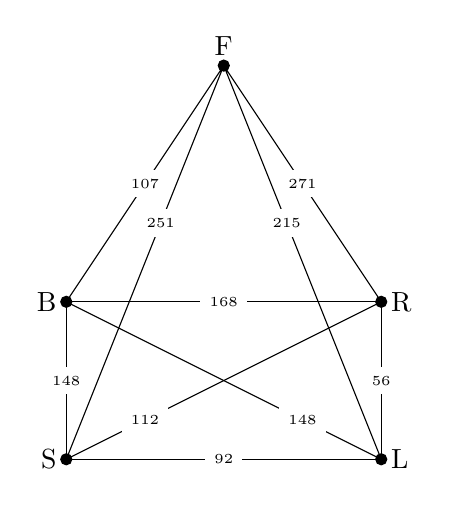
\begin{tikzpicture}
      \filldraw (-2,-1) circle(2pt)
          (-2,1) circle(2pt)
          (2,-1) circle(2pt)
          (2,1) circle(2pt)
          (0,4) circle(2pt);
      \node[anchor=east] at (-2,1) {B};
      \node[anchor=east] at (-2,-1) {S};
      \node[anchor=west] at (2,-1) {L};
      \node[anchor=west] at (2,1) {R};
      \node[anchor=south] at (0,4) {F};
      \draw(-2,-1) --node[pos = 0.5,fill=white]{\tiny 148} (-2,1) --node[pos=0.5,fill=white]{\tiny 168} (2,1) -- node[pos=0.5,fill=white]{\tiny 56} (2,-1) -- node[fill=white,pos=0.5]{\tiny 92}cycle;
      \draw(-2,-1) -- node[pos = 0.25,fill = white]{\tiny 112}(2,1);
      \draw(-2,1) -- node[pos = 0.75,fill=white]{\tiny 148}(2,-1);
      \draw (-2,-1) -- node [pos = 0.6,fill=white]{\tiny 251}(0,4)
        (-2,1) -- node[pos = 0.5, fill=white]{\tiny 107}(0,4)
        (2,-1) -- node[pos = 0.6, fill=white]{\tiny 215}(0,4)
        (2,1) -- node[pos = 0.5,fill=white]{\tiny 271}(0,4);

    \end{tikzpicture}
  \end{center}
  \pagebreak
  \begin{center}
    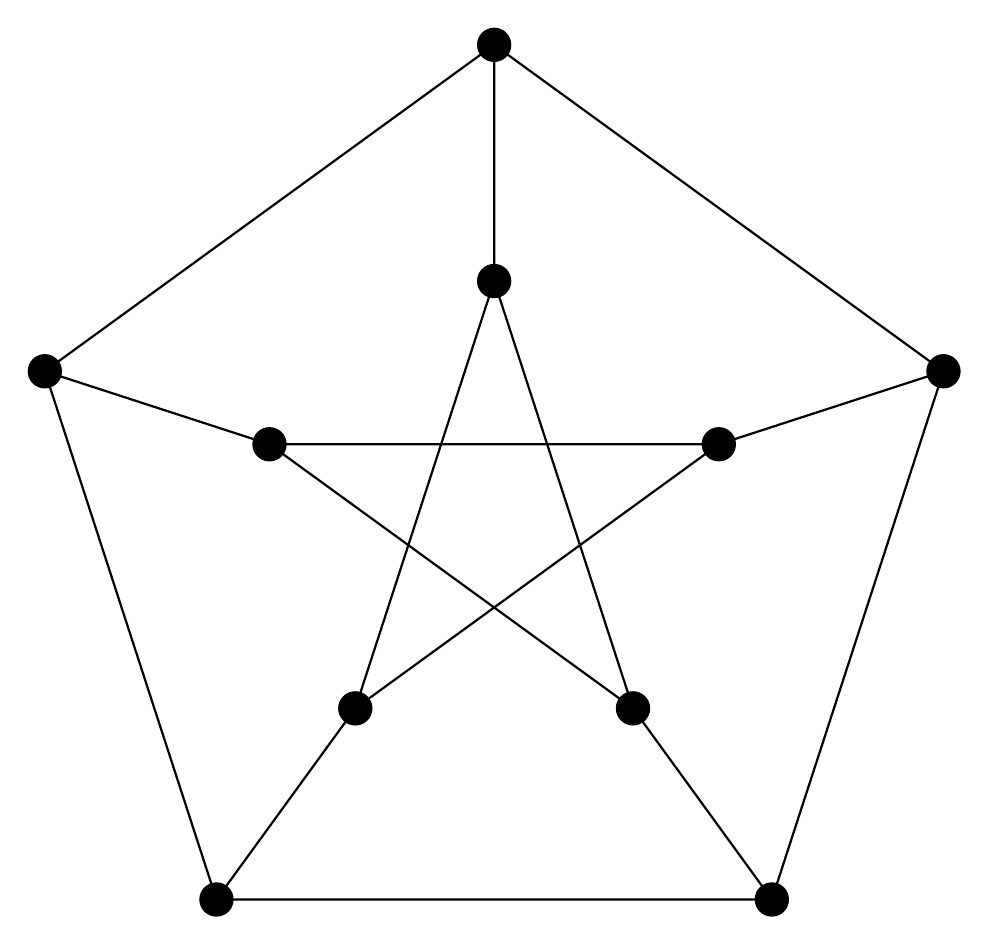
\begin{tikzpicture}[scale = 3]
      \filldraw (18:1cm) circle(2pt);
      \filldraw (90:1cm) circle(2pt);
      \filldraw (162:1cm) circle(2pt);
      \filldraw (234:1cm) circle(2pt);
      \filldraw (306:1cm) circle(2pt);
      \filldraw (18:2cm) circle(2pt);
      \filldraw (90:2cm) circle(2pt);
      \filldraw (162:2cm) circle(2pt);
      \filldraw (234:2cm) circle(2pt);
      \filldraw (306:2cm) circle(2pt);
      \draw[thick] (18:2cm) -- (90:2cm) -- (162:2cm) -- (234:2cm) -- (306:2cm) -- cycle;
      \draw[thick] (18:1cm) -- (162:1cm) -- (306:1cm) -- (90:1cm) -- (234:1cm) -- cycle;
      \draw[thick] (18:2cm) -- (18:1cm)
            (90:2cm) -- (90:1cm)
            (162:2cm) -- (162:1cm)
            (234:2cm) -- (234:1cm)
            (306:2cm) -- (306:1cm);
    \end{tikzpicture}
  \end{center}
}\end{document}
